\documentclass[11pt]{article}
\usepackage[margin=1in]{geometry}
\usepackage{graphicx}
\usepackage{booktabs}
\usepackage{amsmath,amssymb}
\usepackage[numbers,sort&compress]{natbib}
\usepackage{caption}
\usepackage{xcolor}
\usepackage{microtype}
\usepackage{float}
\usepackage[hidelinks]{hyperref}
\captionsetup{font=small,labelfont=bf}
\graphicspath{{figs/}}

\title{Model Diversity Does Not Break the Herd:\\Prompt vs.\ Model Diversity in LLM Agent Populations\\under Shared Information Shocks}

\author{Viren Varma\\
Independent Researcher, Seattle, WA}
\date{November 2026}

\begin{document}
\maketitle

\begin{abstract}
Populations of autonomous agents built on a small number of foundation models may react to the same signal in the same way, amplifying shocks. The usual prescription is diversity: more prompts, more models. We test both forms of diversity head-to-head in a controlled multi-agent market environment. Thirty-six 30-day episodes drawn from 2016--2023 US equity data are replayed under ten agent configurations that differ only in which agents are LLM-driven; on day~10 the LLM agents see either an unverified scary rumor (24 episodes) or neutral placebo news (12 episodes). Prices move with real returns plus the agents' own price impact, and the outcome is the abnormal return relative to the fundamental path, so historical crashes cannot leak into the result. With a single model (Claude Haiku~5.5) the five-day abnormal return after a rumor is $-1.2$, $-1.5$ and $-5.2$ percentage points at LLM shares of 25\%, 50\% and 100\% (bootstrap 95\% CIs exclude zero; share\,$\times$\,rumor interaction $-0.086$, $p<0.001$, standard errors clustered by episode). Placebo news produces no abnormal return. Five prompt personas on the same model halve the full-share effect ($-2.6$\,pp; paired difference $+2.6$\,pp, $p=0.02$). Replacing half of the agents with a second model (DeepSeek~V4.1~Flash) does not dampen the response but amplifies it to $-17.4$\,pp (triple interaction $-0.119$, $p<0.001$): the second model trades in sizes 3--5$\times$ larger and sells on 51\% of rumor days versus 23\% for Haiku. Heterogeneity of models is not heterogeneity of behaviour; what matters is the cross-model correlation of actions under stress. The full study costs about \$60 in API calls and is released with code.
\end{abstract}

\section{Introduction}

Financial regulators have raised the concern that if many market participants delegate decisions to a small number of foundation models, those participants will react to the same signals in the same way and amplify shocks \citep{boe2026}. The implicit remedy is diversity---more prompts, more models, more vendors. Whether diversity actually works is an empirical question that is only beginning to be tested, and the existing evidence is mixed. Agent-based studies mostly use one model, do not include a placebo condition, and report price paths that are hard to separate from the historical data they replay \citep{sok2026,twinmarket2025}. Three recent preprints argue, from different settings, that vendor diversity alone does not reduce correlated behaviour \citep{ross2026,kohli2026,saxena2026}, while laboratory-style cascade experiments find little herding at all \citep{hansen2025,zhang2026}.

This paper contributes a controlled design that addresses these gaps directly and treats the question as one of \emph{evaluating populations of LLM agents}, with a financial market as the test bed:

\begin{enumerate}
  \item \textbf{Paired episodes.} Every configuration replays the same 36 windows with the same seeds; configurations are compared episode by episode.
  \item \textbf{Share-0 control and abnormal-return outcome.} The fundamental path is the real return series and agents only add price impact. The outcome is $\log(1+r^{\mathrm{sim}})-\log(1+r^{\mathrm{fund}})$, so a 2020-style crash in the data cancels exactly.
  \item \textbf{Placebo news.} One third of episodes show neutral news of identical length and structure, separating ``there is news'' from ``the news is scary''.
  \item \textbf{Prompt diversity vs.\ model diversity in the same market.} Arms \textsc{mono} (one model, one prompt), \textsc{persona} (one model, five prompts) and \textsc{mixed} (two models, one prompt) at LLM shares of 0, 25, 50 and 100\%.
\end{enumerate}

The headline result is negative for the monoculture remedy as usually stated: adding a second model did not break the herd, because the second model herded harder.

\section{Related work}

\citet{ross2026} show in homogeneous LLM populations that more capable models behave more alike, that a shared misinformation environment reverses the price-discovery benefit of LLM participation, and that sharing a vendor does not predict correlation; they describe a ``non-diversifiable risk floor''. \citet{kohli2026} find in an agentic wealth-management model that provider diversification has no effect on tail liquidation while de-synchronising execution rules does. \citet{saxena2026} replicate a classic laboratory asset market \citep{hommes2008} with fifteen LLMs and find that mixed-model markets are high-variance and that frontier models adapt to trend-followers rather than stabilise prices. \citet{sok2026} show that a single fake headline produces a flash crash in a growing share of runs as the number of DeepSeek agents rises, and \citet{wang2026fake} benchmark information-injection attacks on single trading agents. On the other side, \citet{hansen2025} and \citet{zhang2026} find that LLM agents in sequential cascade experiments herd less than humans. Surveys \citep{xia2026,scis2026} list ``herding around shared LLM foundations'' as an open direction and call for reproducible protocols. Our design is, to our knowledge, the first to combine a paired share-0 control, a placebo, a dose-response in LLM share and a head-to-head test of prompt versus model diversity in one market; the \textsc{mixed} arm is a direct in-market test of the hypothesis in \citet{ross2026}.

\section{Environment and agents}

\paragraph{Market.} Five assets (SPY, QQQ, XLF, AAPL, NVDA). Each episode is 30 trading days of CRSP daily data between 2016-01-01 and 2023-12-31, with 20 prior days used only to seed volatility. Prices are rescaled to 100 at the start of each episode so that the models cannot infer the calendar date from price levels. Each day the mid price moves by the real (fundamental) return plus price impact:
\begin{align}
\mathrm{impact}_t &= \alpha\,\frac{\mathrm{net\ shares}_t}{L_t}, \qquad
L_t = \frac{D}{(1+2\,\sigma_t)(1+1.5\,|\mathrm{imb}_t|)} \ \ (\text{floored at } 0.1\,D),\\
r^{\mathrm{sim}}_t &= (1+r^{\mathrm{fund}}_t)(1+\mathrm{impact}_t)-1, \qquad
\mathrm{abn}_t = \log(1+r^{\mathrm{sim}}_t)-\log(1+r^{\mathrm{fund}}_t),
\end{align}
with $\alpha=0.25$, $D$ equal to five times the population's aggregate initial holdings of the asset, and daily impact clipped to $\pm 8\%$. If every agent dumped its entire SPY position on one day the impact would be $-5\%$; a single noise trade of 3\% of one agent's wealth moves the price by about 0.015\%. Spreads widen with volatility and order imbalance.

\paragraph{Agents.} 100 agents with log-normal wealth (median \$100k, $\sigma=0.8$, floor \$5k), 50\% invested equal-weight at the start so that selling is possible. Rule-based agents have heterogeneous parameters drawn per agent: fundamental traders (50\%; trade toward a private fair value when the deviation exceeds a threshold $U(0.5\%,3\%)$), trend followers (30\%; sign of the last 3--11 day return beyond $U(1\%,4\%)$) and noise traders (20\%; random trade with probability $U(5\%,20\%)$). A fixed random permutation of agent slots is converted to LLM agents as the share rises, so configurations differ only in who is LLM-driven. Rule agents never see news.

\paragraph{LLM agents.} Every day each LLM agent receives a compact prompt with the five assets' price, 1- and 5-day return, volatility and spread, its own positions, cash and P\&L, and any news. It answers with one line of JSON: a list of \{ticker, BUY/SELL/HOLD, fraction $\le 0.2$ of portfolio value\} and a six-word reason. Thinking/reasoning modes are disabled; temperature is 0 where the API allows; the output budget is 400 tokens. Unparsable replies count as HOLD and are logged (59 of 517{,}500 calls, 0.01\%). Arms: \textsc{mono} uses Claude Haiku~5.5 with one baseline prompt; \textsc{persona} uses Haiku with five prompts (cautious, momentum, contrarian, news-driven, arbitrage) assigned round-robin; \textsc{mixed} uses Haiku and DeepSeek~V4.1~Flash (via OpenRouter) 50/50 with the baseline prompt.

\paragraph{Shock.} On day 10 and the following nine days the LLM agents see one news item drawn from six scary or six placebo templates of identical length and structure. Scary items are explicitly unverified rumors (bank liquidity strain, emergency central-bank meeting, geopolitical escalation, forced fund liquidation, sovereign default, cyberattack on market infrastructure). Placebo items are routine announcements (conference schedule, holiday trading hours, statistical bulletin, index rebalance date). Twenty-four episodes are scary and twelve placebo; windows and assignments are sampled once with a fixed seed and are identical across configurations (Appendix~\ref{app:episodes}).

\paragraph{Outcomes and estimation.} $\mathrm{CAR}^{\mathrm{SPY}}_{k}$ is the cumulative abnormal return on SPY from the event day through day $k$; $\min\mathrm{CAR}_{10}$ is the worst cumulative abnormal return within ten days; sell/buy fractions are unique agents trading per day. Paired effects are outcome minus the share-0 control for the same episode, with bootstrap 95\% CIs over episodes. We also report difference-in-differences (scary minus placebo) and OLS with standard errors clustered by episode: $\mathrm{CAR}^{\mathrm{SPY}}_5 \sim \mathrm{share}\times\mathrm{scary}$ and $\mathrm{CAR}^{\mathrm{SPY}}_5 \sim \mathrm{share}\times\mathrm{scary}\times\mathrm{arm}$ ($n=432$ configuration-episodes).

\paragraph{Scale.} 517{,}500 LLM calls (108{,}000 per full-share run); Haiku~5.5 costs about \$0.000124 per call, DeepSeek~V4.1~Flash about \$0.0001. The valid sweep cost about \$62 and ran in roughly eight hours on a laptop with ten runs in parallel.

\section{Results}

\begin{figure}[t]
  \centering
  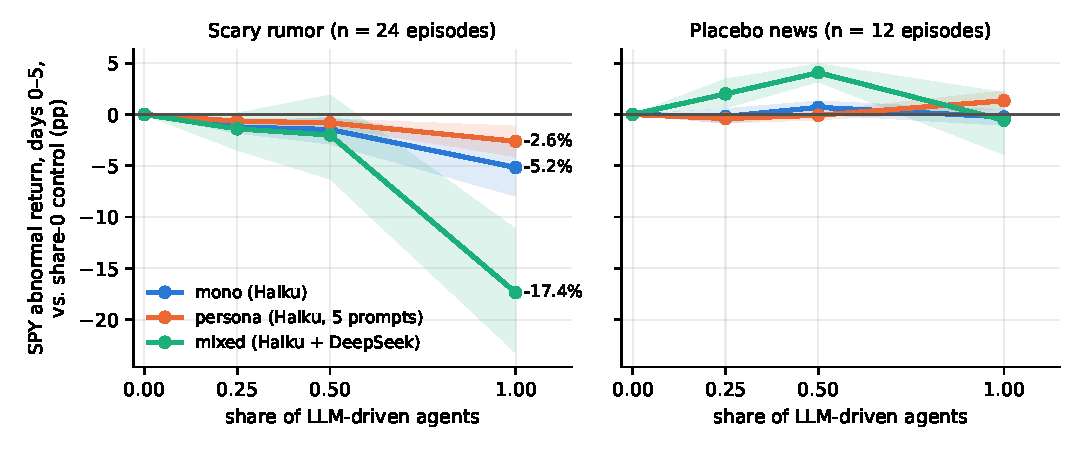
\includegraphics[width=\linewidth]{fig1_dose_response.pdf}
  \caption{Dose-response. Paired five-day abnormal return on SPY versus the share-0 control, by arm and LLM share. Left: scary rumor episodes ($n=24$). Right: placebo episodes ($n=12$). Bands are bootstrap 95\% CIs over episodes.}
  \label{fig:dose}
\end{figure}

\subsection{Rumor response rises with LLM share; placebo is flat}

Table~\ref{tab:paired} and Figure~\ref{fig:dose} give the paired effects. In the \textsc{mono} arm the five-day effect grows monotonically from $-1.2$\,pp at share 0.25 to $-5.2$\,pp at share 1.0, with every CI excluding zero. The control itself is flat: mean $\mathrm{CAR}^{\mathrm{SPY}}_5$ at share 0 is $+0.5$\,pp (s.d.\ 0.9) in both scary and placebo episodes, confirming that the abnormal-return construction removes the historical path. Placebo news produces no effect in \textsc{mono} at any share.

\begin{table}[t]
  \centering\small
  \caption{Paired effects versus the share-0 control, scary episodes ($n=24$), in percentage points with bootstrap 95\% CIs. Last column: placebo episodes ($n=12$).}
  \label{tab:paired}
  \setlength{\tabcolsep}{4pt}\footnotesize
  \resizebox{\linewidth}{!}{%
  \begin{tabular}{llrrrrr}
    \toprule
    Arm & Share & CAR$_2$ & CAR$_5$ & CAR$_{10}$ & $\min$CAR$_{10}$ & CAR$_5$ placebo \\
    \midrule
    mono    & 0.25 & $-1.2$ [$-1.9,-0.6$] & $-1.2$ [$-1.8,-0.7$] & $-0.6$ [$-1.2,-0.1$] & $-1.0$ [$-1.8,-0.3$] & $-0.2$ [$-0.9,+0.6$] \\
    mono    & 0.50 & $-1.8$ [$-3.4,-0.5$] & $-1.5$ [$-2.8,-0.3$] & $-0.0$ [$-1.2,+1.0$] & $-1.7$ [$-3.2,-0.4$] & $+0.7$ [$+0.0,+1.3$] \\
    mono    & 1.00 & $-4.9$ [$-7.9,-2.4$] & $-5.2$ [$-7.9,-2.6$] & $-2.7$ [$-5.5,-0.3$] & $-5.1$ [$-8.1,-2.5$] & $-0.2$ [$-1.1,+0.4$] \\
    \addlinespace
    persona & 0.25 & $-0.6$ [$-0.9,-0.3$] & $-0.7$ [$-1.0,-0.4$] & $-0.4$ [$-0.9,+0.0$] & $-0.4$ [$-0.7,-0.1$] & $-0.4$ [$-0.8,+0.0$] \\
    persona & 0.50 & $-0.8$ [$-1.3,-0.3$] & $-0.8$ [$-1.2,-0.4$] & $-0.4$ [$-1.0,+0.1$] & $-0.8$ [$-1.2,-0.4$] & $-0.1$ [$-0.5,+0.3$] \\
    persona & 1.00 & $-3.2$ [$-4.6,-1.8$] & $-2.6$ [$-4.1,-1.2$] & $-1.0$ [$-2.5,+0.4$] & $-2.9$ [$-4.3,-1.7$] & $+1.3$ [$+0.6,+2.3$] \\
    \addlinespace
    mixed   & 0.25 & $-1.7$ [$-2.9,-0.7$] & $-1.4$ [$-3.4,+0.1$] & $+1.1$ [$-0.9,+2.9$] & $-2.2$ [$-4.2,-0.6$] & $+2.0$ [$+0.6,+3.4$] \\
    mixed   & 0.50 & $-3.2$ [$-6.5,-0.5$] & $-2.0$ [$-6.3,+1.9$] & $+1.4$ [$-2.6,+5.1$] & $-6.2$ [$-10.6,-2.3$] & $+4.1$ [$+3.2,+5.0$] \\
    mixed   & 1.00 & $-15.6$ [$-19.9,-11.0$] & $-17.4$ [$-23.4,-11.4$] & $-12.3$ [$-17.1,-7.7$] & $-23.1$ [$-28.0,-17.9$] & $-0.6$ [$-3.9,+2.2$] \\
    \bottomrule
  \end{tabular}}
\end{table}

\subsection{Difference-in-differences and regression}

Scary minus placebo of the paired five-day effect (Welch $t$ over episodes) is $-1.0$\,pp ($p=0.044$), $-2.2$\,pp ($p=0.008$) and $-4.9$\,pp ($p=0.002$) for \textsc{mono} at shares 0.25, 0.5 and 1.0; $-0.3$ ($p=0.37$), $-0.7$ ($p=0.021$) and $-4.0$\,pp ($p<0.001$) for \textsc{persona}; and $-3.4$ ($p=0.008$), $-6.1$ ($p=0.010$) and $-16.8$\,pp ($p<0.001$) for \textsc{mixed}. Table~\ref{tab:reg} reports the clustered regressions. The share\,$\times$\,scary interaction is $-0.086$ ($p<0.001$) pooled; with arm interactions the \textsc{persona} modifier is small and insignificant ($+0.009$, $p=0.47$) while the \textsc{mixed} modifier is large and negative ($-0.119$, $p<0.001$). Paired within the same 24 scary episodes at full share, \textsc{persona}\,$-$\,\textsc{mono} $=+2.6$\,pp ($p=0.023$) and \textsc{mixed}\,$-$\,\textsc{mono} $=-12.2$\,pp ($p<0.001$). Sign consistency across episodes: \textsc{mono} negative in 18 of 24, \textsc{persona} 19, \textsc{mixed} 20 (Figure~\ref{fig:episodes}).

\begin{table}[t]
  \centering\small
  \caption{OLS on $\mathrm{CAR}^{\mathrm{SPY}}_5$, standard errors clustered by episode, $n=432$. Share-0 control enters once per arm. Reference arm: \textsc{mono}.}
  \label{tab:reg}
  \begin{tabular}{lrrr}
    \toprule
    Term & Coef. & s.e. & $p$ \\
    \midrule
    \multicolumn{4}{l}{\emph{Pooled:} $\mathrm{CAR}_5 \sim \mathrm{share}\times\mathrm{scary}$ \quad ($R^2=0.21$)} \\
    share & $+0.002$ & 0.007 & 0.76 \\
    scary & $+0.005$ & 0.005 & 0.33 \\
    share $\times$ scary & $-0.086$ & 0.017 & $<0.001$ \\
    \addlinespace
    \multicolumn{4}{l}{\emph{By arm:} $\mathrm{CAR}_5 \sim \mathrm{share}\times\mathrm{scary}\times\mathrm{arm}$ \quad ($R^2=0.37$)} \\
    share $\times$ scary (mono) & $-0.050$ & 0.015 & 0.001 \\
    share $\times$ scary $\times$ persona & $+0.009$ & 0.013 & 0.47 \\
    share $\times$ scary $\times$ mixed & $-0.119$ & 0.034 & $<0.001$ \\
    \bottomrule
  \end{tabular}
\end{table}

\begin{figure}[t]
  \centering
  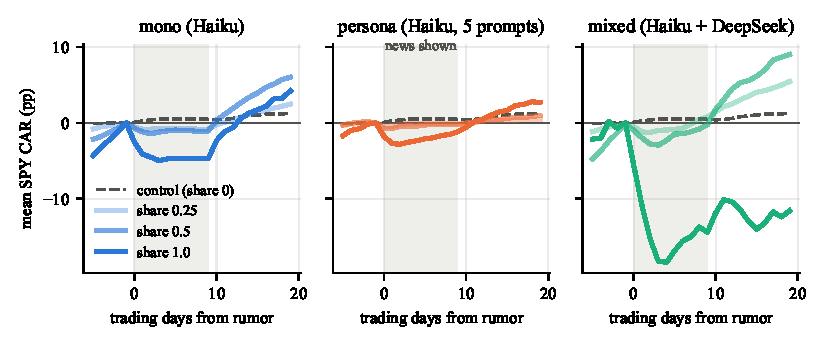
\includegraphics[width=\linewidth]{fig2_car_paths.pdf}
  \caption{Event-time mean SPY cumulative abnormal return in scary episodes, by arm and share; shaded region is the ten-day news window. The \textsc{mono} response is a sell-then-freeze that reverses after the news stops; the \textsc{mixed} response is three times deeper and persists.}
  \label{fig:paths}
\end{figure}

\subsection{Mechanism: who sells, and how much}

Haiku's response is a \emph{sell-then-freeze}: on the rumor day roughly three quarters of Haiku agents sell (peak unique-seller fraction 0.71--0.74 versus 0.21--0.24 before the event), and buying essentially stops for the news window (buy fraction 0.01--0.02 on days 0--2 versus 0.08--0.10 on placebo days). Persona agents keep trading in both directions---the contrarian and arbitrage personas buy into the dip (buy fraction 0.37--0.39)---which is why their net effect is smaller.

Figure~\ref{fig:mixed} decomposes the \textsc{mixed} arm at full share by model. DeepSeek trades almost every day in both directions and in sizes 3--5$\times$ Haiku's: it sells on 41\% of pre-event calls versus 19\% for Haiku, with an average requested sell size of 0.033 of portfolio value versus 0.010. During the news window its sell rate rises to 51\% and its buying halves, in the same direction as Haiku. The two models therefore do not offset each other; the market receives the same sign of pressure with larger volume, and the impact function turns that into a deeper and more persistent dip. The upward placebo drift in the \textsc{mixed} arm at shares 0.25 and 0.5 ($+2.0$ and $+4.1$\,pp) is the mirror image: on quiet days DeepSeek is a net buyer.

\begin{figure}[t]
  \centering
  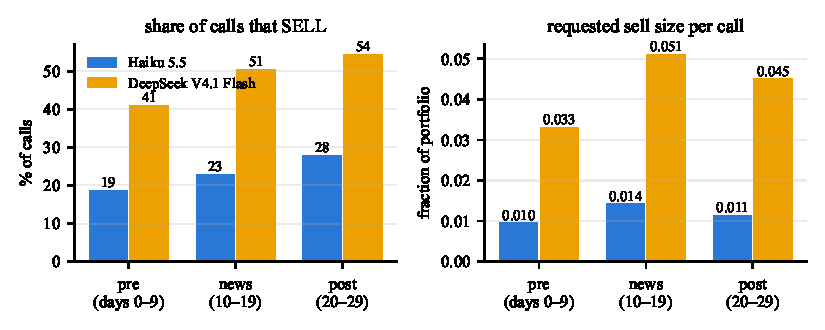
\includegraphics[width=\linewidth]{fig3_mixed_behaviour.pdf}
  \caption{Per-model behaviour in the \textsc{mixed} arm at share 1.0 (all 36 episodes, parsed replies). DeepSeek~V4.1~Flash sells more often and in larger sizes than Haiku~5.5 in every window and moves in the same direction on news.}
  \label{fig:mixed}
\end{figure}

\begin{figure}[t]
  \centering
  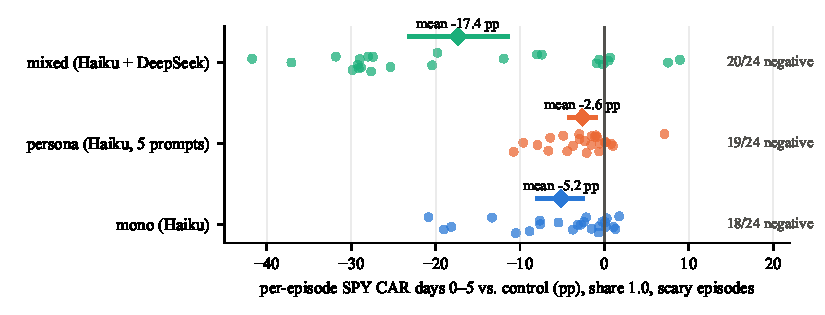
\includegraphics[width=\linewidth]{fig4_episode_effects.pdf}
  \caption{Episode-level paired effects at share 1.0 in the 24 scary episodes. Diamonds and bars are the mean and bootstrap 95\% CI.}
  \label{fig:episodes}
\end{figure}

\section{Interpretation}

\begin{enumerate}
  \item \textbf{Herding is real and dose-dependent.} A market in which a quarter of traders consult the same LLM already shows a $\sim$1\,pp abnormal five-day move on an unverified rumor; a market in which all do shows $\sim$5\,pp. The control and the placebo rule out the two obvious alternatives (history leaking in; an any-news effect).
  \item \textbf{Prompt diversity is a weak mitigant.} Five personas on one model roughly halve the effect at full share and leave the dose-response intact, consistent with the same-model floor of \citet{ross2026}.
  \item \textbf{Model diversity is not a mitigant per se.} What matters is whether the models \emph{disagree in direction} on the shock. Here they agreed; the more aggressive one dominated, and diversity raised the variance of outcomes as well as the mean response. ``Use more vendors'' is therefore not a sufficient prescription. The relevant quantity is the correlation of actions across models under stress, which can be measured with exactly this kind of paired design.
  \item \textbf{The behaviour is prompt-fragile.} In pilot runs the same Haiku agents switched from selling on 72--80\% of rumor days to 0--3\% when the output format required an explicit HOLD per asset (Section~\ref{sec:robust}). Any single number is conditional on the interface the agents are given; the ordering of arms and the dose-response are the robust claims.
\end{enumerate}

\section{Robustness, incidents and limitations}
\label{sec:robust}

\paragraph{Prompt-format sensitivity.} In a pilot with 25 Haiku agents on one scary episode, the share of agents selling on the rumor day was 72--80\% when the output format listed trades with omitted tickers held (the format used in the sweep), 3\% when the prompt added ``if nothing, return an empty list'', and 0\% when an explicit HOLD entry was required per asset. A robustness sweep with the per-asset format is planned and will be reported alongside the main result.

\paragraph{Provider-outage incident.} During the first pass the OpenRouter key hit a pre-set spending limit; every DeepSeek call thereafter returned HTTP~403 and the affected agents were logged as HOLD. The run's circuit breaker required more than 50\% of a step's calls to fail, and one dead provider in a 50/50 arm produced exactly 50\%, so the pass completed silently. The 71 affected \textsc{mixed} episodes were identified from the call logs, quarantined and re-run after the limit was raised; the breaker now trips at 20\% and 401/402/403 responses abort the run. All \textsc{mixed} numbers above come from the clean re-run (0 errors in 139{,}500 calls). We report this because silent degradation of one provider is itself a realistic failure mode for deployed agent populations.

\paragraph{Limitations.} The market is stylised: 100 agents, a linear impact function with a daily cap, no order book and no market makers who could absorb the flow; absolute magnitudes are calibration-dependent while the ordering and the dose-response are not. The \textsc{mixed} conclusion is about these two models; a model that systematically buys on rumors would produce the opposite result, which is exactly the quantity we argue should be measured before relying on diversity. Agents see the same rumor text for ten days with no confirmation or denial, have no memory across days beyond their portfolio, and the rule traders do not see news. Haiku~5.5 and DeepSeek~V4.1~Flash are small, cheap models chosen for budget; the design transfers unchanged to larger ones. Outcomes are reported for SPY; the equal-weight CAR across the five assets gives the same ordering ($-3.8$, $-2.7$ and $-8.9$\,pp at day 5 for \textsc{mono}, \textsc{persona} and \textsc{mixed} at full share).

\section{Conclusion}

In a paired event study with a share-0 control and a placebo, LLM agents over-react to unverified bad news, and the over-reaction grows with the share of LLM agents. Prompt diversity dampens it modestly; model diversity, in the one pairing we tested, amplified it, because the second model traded larger and in the same direction. For the evaluation of multi-agent LLM systems the lesson is that the stability-relevant quantity is the cross-model correlation of actions under stress, not the vendor count. The design and code are cheap enough---about \$60 in API calls---to re-run with any set of models.

\paragraph{Code and data.} Code (\texttt{herd2}), configuration, per-episode outputs and call logs are available at \url{https://github.com/virenvarma007/llm-herding-event-study}. CRSP price data are not redistributed.

\bibliographystyle{plainnat}
\bibliography{refs}

\appendix
\section{Episode windows}
\label{app:episodes}
\begin{table}[H]
  \centering\small
  \caption{The 36 episode windows (start date, event date). Windows are non-overlapping and were sampled once with a fixed seed; the scary/placebo labels were shuffled with the same seed. Episode 19's event day (2020-03-02) sits inside the COVID crash; because the outcome is abnormal return, the crash is in the control and cancels.}
  \setlength{\tabcolsep}{3.5pt}\footnotesize
  \begin{tabular}{llll@{\quad}llll}
    \toprule
    \# & Type & Start & Event & \# & Type & Start & Event \\
    \midrule
    0 & scary & 2016-01-14 & 2016-01-29 & 18 & placebo & 2019-09-27 & 2019-10-11 \\
    1 & scary & 2016-03-21 & 2016-04-05 & 19 & placebo & 2020-02-14 & 2020-03-02 \\
    2 & scary & 2016-08-22 & 2016-09-06 & 20 & scary & 2020-04-28 & 2020-05-12 \\
    3 & scary & 2016-10-14 & 2016-10-28 & 21 & scary & 2020-07-06 & 2020-07-20 \\
    4 & placebo & 2016-12-09 & 2016-12-23 & 22 & placebo & 2020-10-29 & 2020-11-12 \\
    5 & scary & 2017-04-05 & 2017-04-20 & 23 & placebo & 2021-02-12 & 2021-03-01 \\
    6 & scary & 2017-06-08 & 2017-06-22 & 24 & scary & 2021-04-01 & 2021-04-16 \\
    7 & scary & 2017-07-26 & 2017-08-09 & 25 & scary & 2021-08-19 & 2021-09-02 \\
    8 & placebo & 2017-10-23 & 2017-11-06 & 26 & scary & 2021-10-07 & 2021-10-21 \\
    9 & placebo & 2018-02-05 & 2018-02-20 & 27 & scary & 2022-01-06 & 2022-01-21 \\
    10 & placebo & 2018-04-06 & 2018-04-20 & 28 & scary & 2022-04-27 & 2022-05-11 \\
    11 & scary & 2018-05-22 & 2018-06-06 & 29 & placebo & 2022-08-24 & 2022-09-08 \\
    12 & scary & 2018-07-23 & 2018-08-06 & 30 & scary & 2022-10-21 & 2022-11-04 \\
    13 & placebo & 2018-09-17 & 2018-10-01 & 31 & scary & 2022-12-28 & 2023-01-12 \\
    14 & scary & 2018-12-03 & 2018-12-18 & 32 & scary & 2023-03-29 & 2023-04-13 \\
    15 & scary & 2019-04-09 & 2019-04-24 & 33 & placebo & 2023-06-26 & 2023-07-11 \\
    16 & scary & 2019-06-13 & 2019-06-27 & 34 & scary & 2023-09-26 & 2023-10-10 \\
    17 & scary & 2019-08-05 & 2019-08-19 & 35 & placebo & 2023-12-04 & 2023-12-18 \\
    \bottomrule
  \end{tabular}
\end{table}

\section{Configuration}
\begin{table}[H]
  \centering\small
  \caption{Simulation and estimation settings.}
  \begin{tabular}{lp{0.68\linewidth}}
    \toprule
    Agents & 100; rule weights 0.5 / 0.3 / 0.2 (fundamental / trend / noise) \\
    Initial wealth & log-normal, median \$100k, $\sigma=0.8$, floor \$5k; 50\% invested equal-weight \\
    Max single trade & 20\% of portfolio value \\
    Impact & $\alpha=0.25$; depth $=5\times$ aggregate initial holdings; daily cap $\pm 8\%$ \\
    Spread / depth sensitivity & base 5\,bp; volatility 2.0; imbalance 1.5 \\
    Episodes & 36 (24 scary, 12 placebo), 30 days, event day 10, news shown 10 days \\
    LLMs & Claude Haiku~5.5 (thinking off); DeepSeek~V4.1~Flash via OpenRouter (reasoning off, $T=0$); 400 output tokens \\
    Prompt format & free-form trade list; omitted tickers held \\
    Estimation & paired effects with episode bootstrap; OLS with episode-clustered s.e. \\
    Cost & $\approx$\$62 (Haiku $\approx$\$52, DeepSeek $\approx$\$10) for 517{,}500 calls \\
    \bottomrule
  \end{tabular}
\end{table}

\end{document}
